% Template for PLoS
% Version 1.0 January 2009
%
% To compile to pdf, run:
% latex plos.template
% bibtex plos.template
% latex plos.template
% latex plos.template
% dvipdf plos.template

\documentclass[10pt]{article}

% amsmath package, useful for mathematical formulas
\usepackage{amsmath}
% amssymb package, useful for mathematical symbols
\usepackage{amssymb}

% graphicx package, useful for including eps and pdf graphics
% include graphics with the command \includegraphics
\usepackage{graphicx}

% cite package, to clean up citations in the main text. Do not remove.
\usepackage{cite}

\usepackage{color} 



% Use doublespacing - comment out for single spacing
%\usepackage{setspace} 
%\doublespacing


% Text layout
\topmargin 0.0cm
\oddsidemargin 0.5cm
\evensidemargin 0.5cm
\textwidth 16cm 
\textheight 21cm

% Bold the 'Figure #' in the caption and separate it with a period
% Captions will be left justified
\usepackage[labelfont=bf,labelsep=period,justification=raggedright]{caption}

% Use the PLoS provided bibtex style
\bibliographystyle{plos2009}

% Remove brackets from numbering in List of References
\makeatletter
\renewcommand{\@biblabel}[1]{\quad#1.}
\makeatother


% Leave date blank
\date{}

\pagestyle{myheadings}
%% ** EDIT HERE **


%% ** EDIT HERE **
%% PLEASE INCLUDE ALL MACROS BELOW

%% END MACROS SECTION

\begin{document}

% Title must be 150 characters or less
\begin{flushleft}
{\Large
\textbf{Supporting Information}}
% Insert Author names, affiliations and corresponding author email.
\\
Author1$^{1}$, 
Author2$^{2}$, 
Author3$^{3,\ast}$
\\
\bf{1} Author1 Dept/Program/Center, Institution Name, City, State, Country
\\
\bf{2} Author2 Dept/Program/Center, Institution Name, City, State, Country
\\
\bf{3} Author3 Dept/Program/Center, Institution Name, City, State, Country
\\
$\ast$ E-mail: Corresponding maillart@berkeley.edu
\end{flushleft}


\bibliography{../bib/pgame}

\section*{Motivation and Explanation of the Property Crime Mechanism}



\section*{Expected Utility From Strategies and Migration}

{\bf [in this section, we show how individuals use the rules they are endowed with, and how this use changes over time]}

To better determine this ``grain of sand", we resort to simple of economics implied by the property game and opportunities evolve over time: To maximize their payoff, individuals are endowed with three basic rules, 

\begin{itemize}
  \item {\bf strategy update rule:} the player updates its prisoner's dilemma strategy (i.e., cooperate or defect), as a function of her neighbors strategies,
  \item {\bf success driven migration:} the player migrates to the best empty site within her migration area determined by the Moore distance $M$,
  \item {\bf property violation:} the player attempts to expel with probability $s$ another player from her location within their migration area determined by the Moore distance $M$.
\end{itemize}

The three strategies are opportunity based, deterministic for the first two (i.e., if players are presented with better options they will update their strategy or migrate) and random for property violation, reflecting the unsure nature of taking the property of someone else. While decisions are idiosyncratic at the individual level, at the aggregate level, they reveal the expected utility $U$ carried by each rule, which can be formulated as 

\begin{equation}
U_{rule} = p_{rule} \times u_{rule},
\label{U}
\end{equation}

with $p_{rule}$ the probability to execute one of the 3 {\it rules} defined above (i.e., $rule = \{$update, migration, expel$\}$, and $u_{rule}$ the payoff increase from executing a {\it rule}. For prisoner's dilemma strategy update and success-driven migration $p_{rule} = (1~|~u_{rule} > 0)$ (reflecting the deterministic decision to execute these rules) and for property violation $p_{rule} = (s~|~u_{rule} > 0)$, reflecting the unsure nature of attempting to expel another individual. For each rule, $U_{rule}(t)$ provides a direct measure -- at the aggregate level -- of opportunity associated with each rule and how it evolves.

Similarly, one can define an expected mobility distance,

\begin{equation}
N_{rule} = p_{rule} \times n_{rule},
\end{equation}

where $p_{rule}$ is similar as in (\ref{U}) and $n_{rule}$ is the migration distance. $N_{rule}$ shows the expected travel distance for success-driven and property violation migration rules.\\


\subsection*{Population density, Migration Range and Cooperation Level} 
The outcome of the property violation game is nevertheless constrained by the initial conditions, such as population density and migration range: Increased population density reduces the opportunities to find an empty location, and thus, mechanically increases the odds of property violation. The migration range on the one hand increases the chances to find an empty sweet spot in case of success-driven  or forced migrations. On the other hand, it also increases opportunities for property violators. Migration influences the capability by defectors to penetrate clusters of cooperators. However, expelled cooperators can move far enough to make the cluster move away from the defector. Hence, larger migration ranges increase tolerance to property violation (see Figure \ref{fig:phase_transition}b), but their beneficial effects are limited for highly densely populations. On the contrary, populations with very short migration ranges -- here, embodied by unitary migration distance ($M=1$) -- can hardly stand any property violation. 


\subsection*{Optimizing for Property Violation is Managing at the Edge of Collapse}
{\bf [economic argument here]}
Property enforcement is costly, and thus, there is an incentive to limit enforcement to the strict minimum, which will ensure high cooperation (which is equivalent to decide how much property crime a society can stand). For large enough migration ranges ($M\geqslant 3$), a little property violation ($s < 1 \%$), brings the necessary randomness that reduces friction and enhances cooperation, similarly to previous results obtained with other types of noise involved in success-driven migration games \cite{helbing2009outbreak}. For larger property violation $s > 1\%$, cooperation decreases linearly according to $ c = 1 - 2.2\cdot s$, until a critical phase transition is reached (see Figure \ref{fig:phase_transition}a), which itself depends on the population density and the migration range as reported on Figure \ref{fig:phase_transition}b. There is no hard limit, but rather a transition from sure striving society with high cooperation to a sure collapse. The region in between is large compared to the absolute value of the upper limit: For instance, for $M=5$ and $d=0.5$, the phase transition spans from $s = 3.7\%$ to $s= 4.2\%$, with an equal chance to survive or collapse for property violation $s=4\%$. Hence, the ``danger zone" spans over more than 10\% of the limit value, and the decreasing probability of striving in the critical phase transition region, makes it very hard to determine whether the course of a society will end up positively or negatively.\footnote{We have verified that the outcome is independent from the initial grid organization, by running multiple simulations from the same initial grid.}

Starting from a population randomly scattered across the grid with an even number of cooperators and defectors, $U$ and $N$ undergo significant changes over time, with subtle yet determinant differences between a striving and a collapsing society (see Figure \ref{fig:tseries} for an illustration of a successful and a failed outcome with similar parameters $d=0.5$, $M=5$ and $s=0.037$; This particular case illustrates similar stylized facts obtained for different values of $d$, $M$ and $s$). In both the successful and the failed dynamics, {\it success-driven} migration provides the highest expected payoff increase ($U_{migration} > U_{update} > U_{expel}$)  in the early iterations $t < 1.5\times10^{5}$ (over $20\times10^6$ MCS iterations). After $t > 1.5\times10^{5}$, a significant change occurs: In striving societies (Figure \ref{fig:tseries}b) a switch of expected payoff occurs, which becomes : $U_{expell} > U_{update} > U_{migration}$, while in the failed society case (Figure \ref{fig:tseries}b), strategy update provides the highest expected increased payoff, and the expected increased payoff from success-driven and property violation migrations converge.\footnote{ nb: It is important to note that expected payoff is not necessarily increasing overall the entire population: players expelled from their site suffer a negative expected payoff increase (not shown), as well as neighbors around the focal player who changes prisoner's dilemma strategy to defect, or a defector migrating or performing a property violation.} At the time of the switch, we observe an inflection point of the cooperation level (purple dashed circle on Figure \ref{fig:tseries}b): After this point, cooperation still increases in the failed case, but at much lower pace,\footnote{Mostly driven by strategy updates, which provide the highest expected payoff increase? These updates are at first of the type : $D \rightarrow C$ and then, after the peak rather $C \rightarrow D$. The intuition is that, somewhen migration (whether success driven or property violation) does bring enough payoff increase, compared to strategy update, therefore something weird occurs which is that cooperation increases (more or larger clusters?), which in turn prepare for an invasion of defectors!} on the contrary to striving societies for which we observe a smooth continuous increase of cooperation, up to saturation and stabilization at a high level ($c > 0.8$). In the failed scenario illustrated in Figure \ref{fig:tseries}, the peak of cooperation is reached at  $t \approx 5\times10^5$, and collapse occurs after roughly$10^6$ iterations, nearly $850,000$ iterations after the switching point!\\

While it is hard to observe the detailed switching mechanisms occurring at the transition point,\footnote{This may be done in the future.} we find that the expected mobility (the probability to remains high in the failed scenario in comparison with the successful case (Figures \ref{fig:tseries}c and \ref{fig:tseries}d).\footnote{It is important to note that mobility by property violation and consecutively by individuals forced to move, is not nearly as large as the mobility induced by success-driven actions (c.f., Figures \ref{fig:tseries}b Inset 2).} Also, we find that in the successful scenario, a strong decoupling between expected payoff increase occurs (Figures \ref{fig:tseries}a inset 1), while for the collapsing scenario, dependence between expected payoff remain high and get even reinforced (Figures \ref{fig:tseries}b inset 2).\footnote{The correlogram before the switch also shows high dependence (not shown here), which is natural somehow, as the system gets organized {\bf [This correlogram (pre-switching) should be shown too, at least in the supplementary materials. In the failing scenario, it shows that property violation may influence ]}} Moreover, in the latter case, success-driven migration actions strongly drive private property violations (green correlogram) and strategy updates (red correlogram).\footnote{The correlation peak occurs for a negative lag (roughly 15-20 bins {\bf [I must check the size of a bin in terms of iterations]}) when considering the influence of private property violations and strategy updates on migration} Dependence between property violation and strategy update is also high (blue correlogram), but with no lag thus one cannot say whether $E \rightarrow U$ or $U \rightarrow E$. One can infer however that they are both influenced by success-driven migration (see red and green correlograms).\footnote{It is unclear however what makes success-driven migration the driver of other actions. Something special must occur before or at the switching point.}\\

Past the very first iterations where success-driven migration is the predominant way to increase payoff (in order to build and reach clusters of cooperators, regardless of whether the moving player is a cooperator or a defector), our findings draw two completely different stories leading to either collapse or well-established cooperative societies. In the latter scenario, expected payoff from success-driven migration rapidly decays to a level comparable to the expected payoff derived from strategy update and property violation. Additionally expected payoff increase from the three rules get highly independent: A spatio-temporal decoupling occurs and players no longer undergo long-range migration, and while property violation brings the highest expected payoff increase, it is tackled by some kind of locally established self-organization \footnote{(which remains to be explained/documented in further details)}. On the contrary, the collapse scenario is driven by long-range migrations,\footnote{We need perhaps more insights on the nature of these migrations, e.g., do they spread defectors or rather cooperators? Does this evolve over time?} which in turn trigger strategy updates and property violation.\footnote{These long-range spatio-temporal dependences look like systemic risk to me, which may appear in a seamless, subtle and hardly noticeable way!} \footnote{It would be interesting to check the dynamics with a residual level of property violation, e.g., $s=0.01$, and with a super high level of $s$, to see if these extreme cases magnify differences between success and failure.}

\section*{Enduring and Adaptive Societies Facing Property Violation}
One striking observation is that even though the system switches early on, and determines the final outcome, changes may remain unnoticed for a while, as cooperation increases for 4 times more iterations (since $t=0$) until collapse actually occurs.\footnote{In some simulations, the inflection point in the increase of cooperation is hardly noticed (e.g. Figure \ref{fig:adaptation})}\\

Thus, on the one hand it may take time to realize that a society is running towards the edge of collapse, and on the other hand, it may take time to take corrective action, such as taking actions to reduce private property violations.\footnote{As a result of Figure \ref{fig:phase_transition}b, one could also think of increasing migration ranges (which would require massive and long-term infrastructure investments) and decreasing population density, which concretely in our world would mostly require reducing population and would be ethically questionable. Here, we limit our study to private property violations as the main control parameter.}\\

Budgets allocated to property right enforcement may vary over time, in particular, a typical situation is that property crime is low and therefore there is a reduced sense of urgency and budgets might be reduced as a consequence. Also on the long term, institutions concerned with property enforcement may experience downturns of efficiency (e.g., through some kind of corruption).\\

Here, we ask two questions:  

\begin{enumerate}
  \item {\bf Resistance:} Given that a cooperative society is in the process of establishing \footnote{I am currently running simulations for this.} or has stabilized at a high level of cooperation (given a level of property violation), how much more property violation and for how long can this society stand a higher level of property violation?
  \item {\bf Adaptation:} Given that a society is on the path to collapse (as shown e.g., on Figure \ref{fig:tseries}b), how early and by how much property violation shall be reduced to ensure it will strive by reaching a stable high level of cooperation?
\end{enumerate}

\paragraph{Resistance:} We find that when a society has stabilized at a high cooperation level ($s=4\%$), increasing a property violation a little ($0.05 \leqslant s \leqslant 0.06$) increases the chance that cooperation will collapse suddenly yet on the long run ( iterations > $3 \times 10^5$ after change of property violation level). For higher levels of  property violation ($s>0.06$), the cooperation curves decreases in a more or less parabolic shape, which seems to be invariant in the limit of $s \rightarrow \infty$, and it looks like that the zero-cooperation level can be hit at earliest around $3 \times 10^5$ after the increase of property violation (see Figure \ref{fig:resistance}).

\paragraph{Adaptation:} The tipping point  ($t \approx 10^5$) occurs way before the edge of actual collapse ($t \approx 10^{5.7}$), and thus, a very natural question is whether it is possible to take corrective actions to prevent the collapse of cooperation once the tipping point has passed and has 
been detected. We find that unless property violation can be reduced drastically (e.g., 75\%, c.f., Figure \ref{fig:adaptation}d), action must be taken at latest when cooperation is at its maximum  to ensure resilience (see Figure \ref{fig:adaptation}c when property violation is halved). For more realistic property violation reduction (10\% to 25\%, c.f. Figures \ref{fig:adaptation}a and\ref{fig:adaptation}b), the policy maker must intervene as the cooperation still increases. We could of course imagine more complicated and progressive property violation mitigation schemes (which is actually more relevant for drastic actions to reduce of property violation that may take time to take effect), but the idea is that in order to avoid collapse, action must be taken {\bf before} the effects of property violation get actually widely noticed.\footnote{with more simulations, we could actually compute thoroughly the odds of survival given timing and effort deployed to reduce property violation, but I think what is presented here is enough to demonstrate that it is super important to avoid doing what politicians do -- or are forced to do by the ``real-politics" democratic mechanisms, which is taking action only when the problem get sufficiently noticeable by the population.}\\




\section*{Tipping Point and Systemics risks}







\begin{figure}[h!]
\begin{center}
\centerline{\includegraphics[width=7cm]{../figures2/migration_diagram.eps}}
\caption{Migration diagram for focal player (defector on crossed site with $\text{payoff} = 1.3$). The best site in the migration range has highest payoff for the focal player (red-green site with $\text{payoff} = 1.3 \times 4 = 5.2$). The target site with highest payoff is occupied by a cooperative player and may be expelled with probability $s$ (orange arrow). In this case, the player on the target site is forced to move to the nearest empty site with $\text{payoff} = 2$ (black arrow pointing to light green site). However, with probability $1-s$, the focal player moves to the best empty site with $\text{payoff} = 2.6$ (blue arrow pointing to light green site).}
\label{fig:migration_diagram}
\end{center}
\end{figure}


\begin{figure}[h]
\begin{center}
\centerline{\includegraphics[width=16cm]{../figures2/phase_transition_d05.eps}}
\caption{{\bf a.} Phase transition of cooperation levels for migration Moore distances $M = \{1,3,5,7,11\}$ and population density $d=0.5$. For all migration ranges, a small level of property violation $s < 0.5\%$ enhances cooperation, while more property violation decreases cooperation. For $M=1$, cooperation decreases continuously as property violation grows (up to $s = 2\%$). For larger migration ranges, cooperation exhibits a linear decrease (given by $c \approx 1 - 2.2 \cdot s$) up to a critical phase transition point $s^*$. As $M$ increases, $s^{*}$ becomes a range of values (colored areas show the 1st to 99th percentile confidence intervals), where cooperation can either be sustained at high level ($c > 0.8$), or collapse as a result of a stochastic process: in this phase transition region, the outcome is independent of initial grid configuration. For instance, the critical phase transition range for $M=5$ (magenta area) is $3.7\% < s^{*} < 4.2\%$. While the outcome can either be high cooperation or collapse, the probability of high cooperation decreases within the critical phase transition range (cf.\ solid lines within areas): it becomes more likely that cooperation will collapse as property violation reaches the upper boundary of the critical range. {\bf b.} Phase transition areas as a function of population density: for each migration range represented by colored areas, the lower (dashed) boundary shows the limit below which cooperation thrives systematically ($c > 0.8$), while the upper (dash-dotted) boundary shows the limit beyond which cooperation collapses systematically. Larger migration ranges increase significantly the resistance to higher levels of property violation. However, the beneficial effects of long-range mobility are reduced for more densely populated worlds. Short-range mobility ($M=1$) is highly sensitive to property violation, regardless of population density.}
\label{fig:phase_transition}
\end{center}
\end{figure}


\begin{figure}[h]
\begin{center}
\centerline{\includegraphics[width=15cm]{../figures2/tseries_transition_3.eps}}
\caption{Evolution of expected payoff from player actions -- success-driven migration (green), property violation (blue), or strategy update (red). Expected payoff dynamics are initially very similar ($t< 10^5$ iterations) between thriving cooperation ({\bf a}) and collapse ({\bf b}) (same initial conditions: $d=0.5$, $M=5$, $s = 0.037$; colored areas show the 25\%--75\% percentile ranges). At $t \approx 10^5$ iterations, structural changes occur that determine the outcome: although cooperation continues to increase until $t \approx 5\times 10^5$, in the non-sustainable case ({\bf b}) strategy update (red) yields the highest expected payoff, while in the sustained cooperation case ({\bf a}), strategy update never provides the highest expected payoff. In the latter case, a subtle crossing occurs at the transition point $t \approx 10^5$, where migration transitions from the action with highest payoff to a lower payoff, while property violation becomes the action with highest expected payoff. Insets {\bf 1} and {\bf 2} show the correlograms between expected payoffs after the tipping point: in the sustainable case ({\bf a}), cross-dependence is very low, indicating strong decoupling between expected payoffs from different actions. In the collapsing scenario, cross-dependence remains high, with migration causing more property violation (green correlogram) and more strategy updates (red correlogram). In the unsustainable scenario, cooperation still increases long after the tipping point (until $t \approx 5\times10^{5}$) and then abruptly collapses. Panels {\bf c} and {\bf d} show expected mobility distance from success-driven migration (green), property violation (blue), and forced move (cyan). In the collapsing scenario ({\bf d}), expected mobility reaches a high plateau ($\log_{10} U_{\text{mobility}} \approx 2.5$), while for thriving societies ({\bf c}), expected mobility is lower ($1.5 < \log_{10} U_{\text{mobility}} < 2$), close to that of property violators ($\log_{10} U_{\text{expel}} \approx 1.5$). The dynamics presented for $d=0.5$ and $M=5$ are representative of phase transitions occurring for any game with $M>1$ and density $0.2 \leqslant d \leqslant 0.8$.}
\label{fig:tseries}
\end{center}
\end{figure}


\begin{figure}[h]
\begin{center}
\centerline{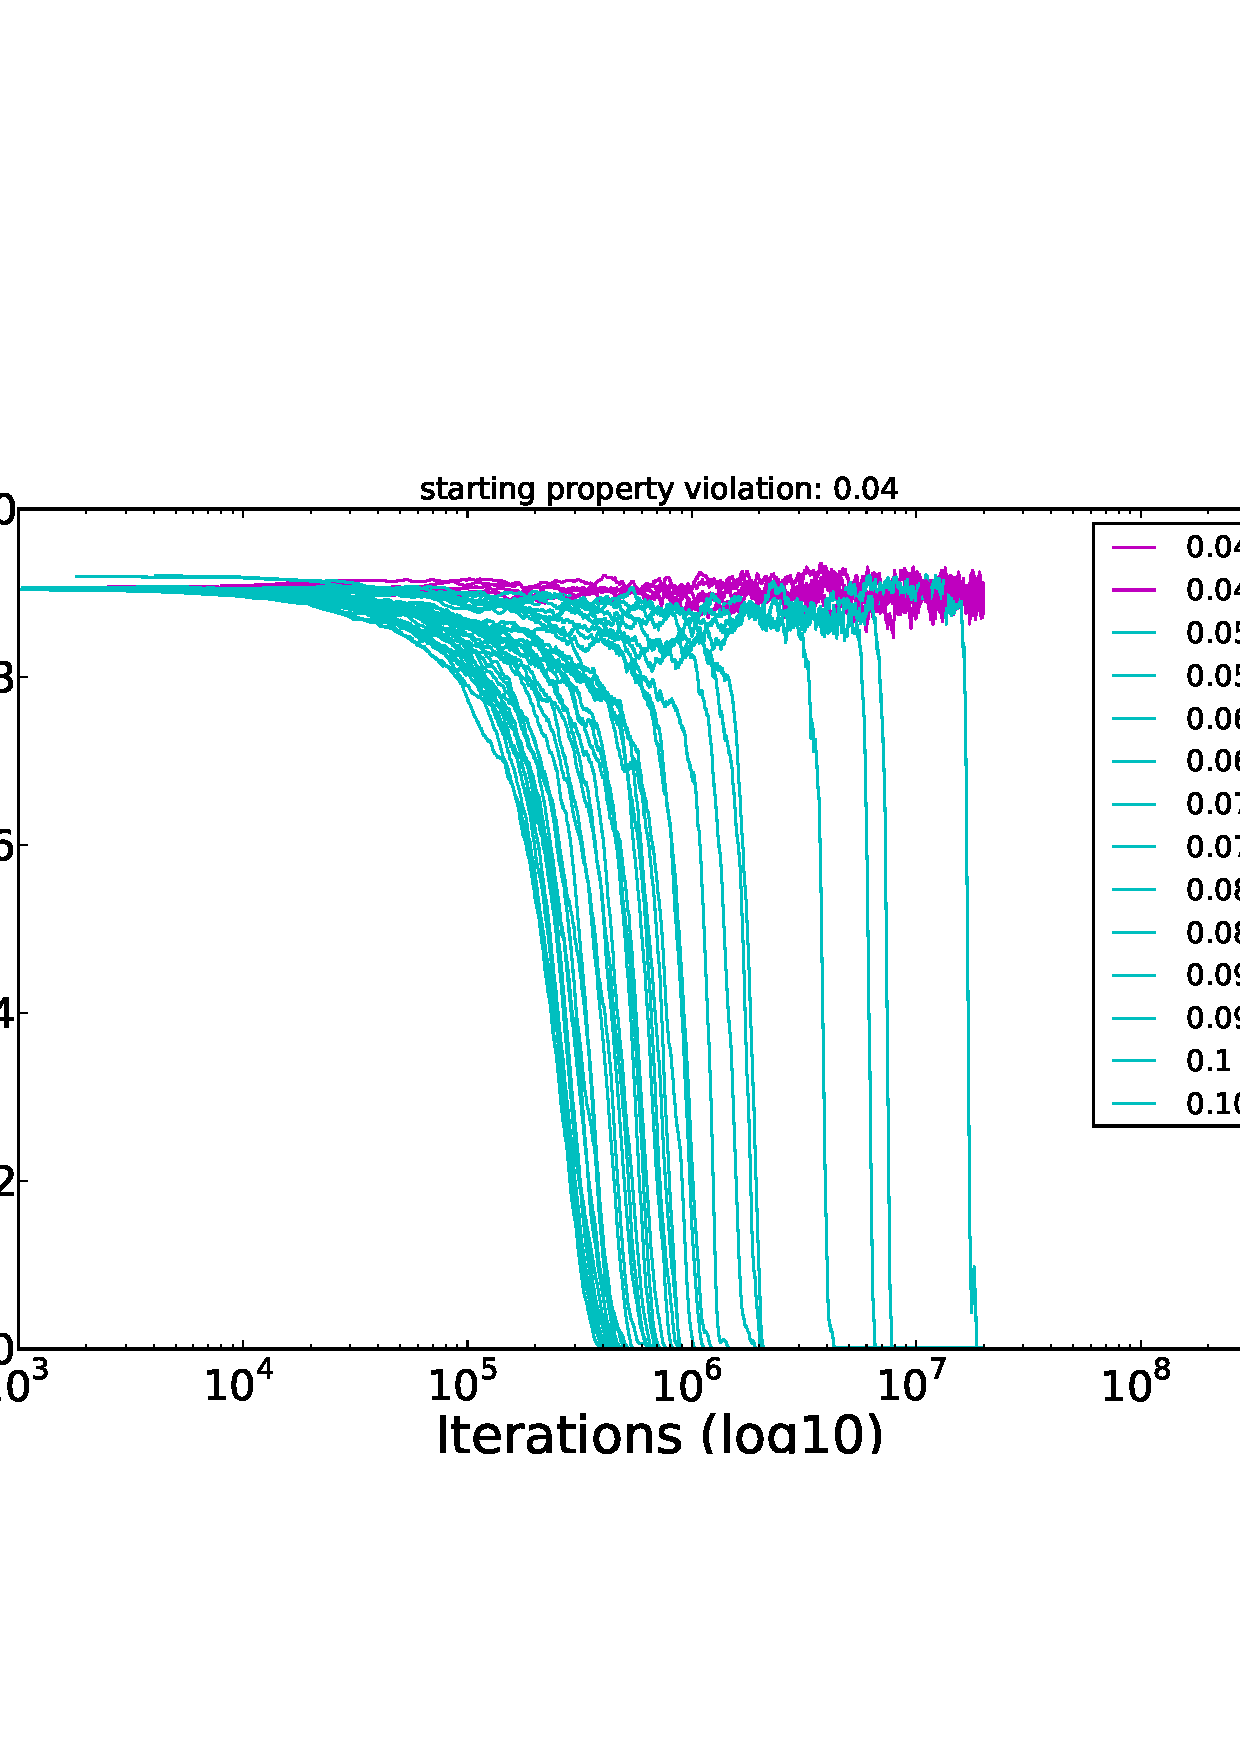
\includegraphics[width=11cm]{../figures2/resistance004.png}}
\caption{Evolution of cooperation when property violation is increased, starting from a simulation stabilized at high cooperation level ($c > 0.8$) and property violation in the upper range of the phase transition ($s=0.040$). For $s < 0.045$, cooperation remains high. For $0.05 \leqslant s \leqslant 0.06$, cooperation may collapse suddenly after $3\times10^6$ iterations, suggesting that any property violation value above the phase transition region may trigger collapse given enough time. For $s>0.06$, the cooperation curve decreases in a roughly parabolic shape that appears invariant in the limit of large $s$. The earliest that cooperation reaches zero is approximately $3 \times 10^5$ steps after the increase in property violation, indicating that even under large increases, a time window remains for corrective intervention.}
\label{fig:resistance}
\end{center}
\end{figure}



%\section*{Tables}
%\begin{table}[!ht]
%\caption{
%\bf{Table title}}
%\begin{tabular}{|c|c|c|}
%table information
%\end{tabular}
%\begin{flushleft}Table caption
%\end{flushleft}
%\label{tab:label}
% \end{table}

\clearpage

%

\section{Social Rule Violation Game Step-by-Step}
\label{stepbystep}

Here, we present a detailed explanation of the decision process involved in the social rule violation game, at each Monte Carlo Step: 

\begin{enumerate}
  \item {\bf Player selection:} At each Monte Carlo Step $MCS$, a site is selected ($MCS = N \times L^2$ with $N$ the number of iterations, and $L$ the side of the square grid). If the site is occupied, the {\bf focal individual} is selected. Each individual is expected to be selected $d \times N$ times with $d$ the grid density. 
  
  \item {\bf Exploration:} With probability $1 - m$, the focal individual strategically explores its own migration (Moore) neighborhood $(2M + 1) \times (2M + 1)$ of range $M$, searching for a site with better payoff given current prisoner's dilemma (PD) strategy, i.e., either cooperate or defect. To assess for sites with best payoff, the individual plays the prisoner's dilemma with her own strategy and with neighbors for each site within the migration neighborhood. For each site assessed, the ``virtual'' payoff is computed as the sum of outcomes from playing the prisoner's dilemma with all neighbors.
  
  \item {\bf Move to best empty location (success-driven migration):} If among the sites with highest payoff, some are empty, the individual moves to the closest empty site.
   
  \item {\bf Move to best occupied location (social rule violation):} If there is no empty site among those with highest payoff, the focal individual expels the target individual with probability $s$. The expelled target individual is forced to move to the closest empty location with highest payoff within her own migration range. The expelled individual may find a new empty site with either lower or higher payoff. For both the focal and the target individual, in case multiple sites with highest payoff are available, the closest one is automatically selected. If they are at the same distance, one site is randomly chosen among best sites with smallest migration distance.
  
  \item {\bf Move to better empty location (success-driven migration):} If there is no empty site among those with highest payoff and property violation did not occur with probability $1-s$, the focal individual moves to the closest empty location with higher -- yet not highest -- payoff.
  
  \item {\bf No migration:} If all empty sites in the migration range have a payoff worse than the incumbent payoff on the focal site, the individual does not move.
   
 \item {\bf PD strategy imitation:} Whether it has moved or not, the individual is allowed to update her PD strategy (cooperate or defect) by playing the prisoner's dilemma with her neighbors. If one neighbor's strategy leads to a better payoff, the focal individual imitates this strategy with probability $1-r$. With probability $r$, her strategy is reset: the individual cooperates with probability $q$ and defects with probability $1-q$. If the target individual is forced to move after a property violation, she is not allowed to update her strategy (because it is not her turn to play). In this study, we consider no imitation noise (i.e., $r=0$). Hence, individuals {\it systematically} copy a more successful PD strategy.
\end{enumerate}

\begin{figure}[h!]
\begin{center}
\centerline{\includegraphics[width=7cm]{../figures2/migration_diagram.eps}}
\caption{Migration diagram for focal player (defector on crossed site with $\text{payoff} = 1.3$). The best site in the migration range has highest payoff for the focal player (red-green site with $\text{payoff} = 1.3 \times 4 = 5.2$). The target site with highest payoff is occupied by a cooperative player and may be expelled with probability $s$ (orange arrow). In this case, the player on the target site is forced to move to the nearest empty site with $\text{payoff} = 2$ (black arrow pointing to light green site). However, with probability $1-s$, the focal player moves to the best empty site with $\text{payoff} = 2.6$ (blue arrow pointing to light green site).}
\label{fig:migration_diagram}
\end{center}
\end{figure}


\section{Simulation Parameters}

All simulations are performed on a two-dimensional square lattice with periodic boundary conditions and side length $L = 200$ (i.e., $40{,}000$ sites). Population density $d$ is set at initialization by randomly occupying a fraction $d$ of sites. At initialization, each occupied site is assigned a cooperator or defector strategy with equal probability ($c_0 = 0.5$). Each individual is updated on average $N = 200$ times over the course of a simulation, yielding a total of $MCS = N \times d \times L^2$ Monte Carlo Steps. The prisoner's dilemma payoff parameters are set to $T = 1.3$, $R = 1$, $P = 0.1$, $S = 0$, satisfying the conditions $T > R > P > S$ and $2R > T + S$. Migration probability is $m = 1$ (no random migration), imitation noise $r = 0$, and random mutation $q = 0$. The key parameters varied across simulations are:
\begin{itemize}
  \item Population density: $d \in \{0.2, 0.3, 0.4, 0.5, 0.6, 0.7, 0.8\}$
  \item Migration range (Moore neighborhood): $M \in \{1, 2, 3, 5, 7, 9, 11, 15, 20\}$
  \item Social rule violation probability: $s \in [0, 0.2]$
\end{itemize}
For each parameter combination, multiple independent simulations are run with different random seeds to capture the stochastic variability of outcomes, particularly near the phase transition.


\section{Emergent Compliance: Why Only Defectors Violate}
\label{behaviors}

An emergent property of the social rule violation game is that cooperators never commit social rule violations, even though the model imposes no such constraint. This arises from the payoff structure of the game in combination with the spatial organization of clusters.

Consider a cooperator occupying a site in a cooperative cluster. Her current payoff is high because she interacts primarily with other cooperators ($R = 1$ per cooperator neighbor). The sites with highest payoff in her Moore neighborhood are similarly embedded in cooperative clusters and are already occupied by cooperators. There are two cases: (i) the best site is empty -- in which case the cooperator migrates there via success-driven migration, not social rule violation; or (ii) the best site is occupied by another cooperator -- in which case expelling that cooperator would not improve the focal cooperator's payoff, as the target site's neighborhood structure is similar to the current one. Hence, cooperators have no payoff incentive to expel incumbents.

By contrast, a defector surrounded primarily by other defectors receives low payoffs ($P = 0.1$ per defector neighbor). Sites adjacent to cooperative clusters offer substantially higher payoffs (up to $T = 1.3$ per cooperator neighbor). These high-payoff sites are typically occupied by cooperators. The defector thus has strong incentive to expel the incumbent cooperator and take the high-payoff site. This asymmetry in incentive structure ensures that, in practice, only defectors attempt and commit social rule violations.


\section{Expected Utility of Playable Strategies}
\label{exp_utility}

To characterize the dynamics of the tipping point, we measure the expected utility of each playable strategy over time. For each Monte Carlo Step, the action taken by the focal individual is recorded along with the resulting payoff change. We define the expected utility $U_k(t)$ of strategy $k$ (where $k \in \{\text{migration}, \text{PD update}, \text{violation}\}$) within a time window $[t - \Delta t, t]$ as:
\[
U_k(t) = \sum_{i \in \text{events}(k, [t-\Delta t, t])} \Delta \pi_i
\]
where $\Delta \pi_i$ is the payoff change resulting from event $i$, and the sum runs over all events of type $k$ within the time window. This measure captures both the frequency with which a strategy is played and the average payoff it yields: a strategy that is played often but yields small payoff changes may have the same expected utility as one played rarely but yielding large changes.

The time window is set to $\Delta t = 1000$ Monte Carlo Steps. The expected utility is computed separately for success-driven migration, PD strategy updates (cooperate $\leftrightarrow$ defect), and social rule violations (including both successful expulsions and failed attempts). By tracking the ordering of $U_{\text{migration}}$, $U_{\text{PD update}}$, and $U_{\text{violation}}$ over time, we identify the tipping point as the moment when this ordering switches.


\section{Expected Mobility}
\label{exp_mobility}

Similarly to the expected utility, we measure the expected mobility to characterize how far individuals move over the course of the simulation. For each migration event (success-driven or violation-induced), we record the Euclidean distance $d_i$ traveled by the focal individual. The expected mobility $E_{\text{mob}}(t)$ within a time window $[t - \Delta t, t]$ is:
\[
E_{\text{mob}}(t) = \frac{1}{|\text{events}|} \sum_{i \in \text{events}([t-\Delta t, t])} d_i
\]

In the thriving regime, expected mobility decreases over time as cooperators settle into stable clusters and move only locally (within the immediate neighborhood). In the collapse regime, expected mobility remains high, reflecting the large-scale displacement of cooperators fleeing from invading defectors. The contrast between local (low-mobility) dynamics in the thriving regime and systemic (high-mobility) dynamics in the collapse regime is a key diagnostic of the tipping point.


\section{Detecting the Tipping Point}
\label{tippingpoint}

The tipping point is identified by monitoring the cross-correlation structure between the expected utilities of the three playable strategies. In the early phase of the simulation ($MCS < 10^5$), the expected utilities of migration, PD update, and violation are positively correlated and their ordering is consistent: $U_{\text{violation}} \leqslant U_{\text{PD update}} \leqslant U_{\text{migration}}$.

At approximately $MCS \approx 10^5$, the dynamics diverge:
\begin{itemize}
  \item In the {\bf thriving regime}, the cross-correlations between expected utilities drop sharply, indicating that the three strategies become {\it decoupled}. Migration, strategy update, and violation operate largely independently, reflecting the fact that small cooperative clusters manage violations locally without systemic repercussions. The expected utility ordering switches to $U_{\text{migration}} \leqslant U_{\text{PD update}} \leqslant U_{\text{violation}}$.
  \item In the {\bf collapse regime}, the cross-correlations remain high, indicating that the strategies remain {\it coupled}. A violation triggers migration, which triggers strategy updates, creating a positive feedback loop. The expected utility ordering switches to $U_{\text{violation}} \leqslant U_{\text{migration}} \leqslant U_{\text{PD update}}$, reflecting the dominance of mass strategy switching from cooperation to defection.
\end{itemize}

The decoupling/coupling diagnostic can be computed from the lag cross-correlation coefficients between $U_{\text{migration}}(t)$, $U_{\text{PD update}}(t)$, and $U_{\text{violation}}(t)$ evaluated after the regime switch (see Figure \ref{fig:tseries}, insets 1 and 2).


\section{Resilience and Hysteresis}
\label{resilience}

To test the hysteresis properties of the social rule violation game, we start from a limit case ($d = 0.5$, $M = 5$, $s = 4.2\%$) where cooperation is known to collapse after approximately $10^6$ Monte Carlo Steps. At various time points after the tipping point ($t^* \approx 10^5$ iterations), we reduce the violation probability $s$ by a fixed percentage ($10\%$, $25\%$, $50\%$, or $75\%$) and observe whether cooperation recovers. Results are shown in Figure \ref{fig:adaptation} (main text).


\clearpage


\subsection*{Parameter Interpretation}

The rationale for varying the population density stems from the intuition that densely populated areas are more resource-intensive (i.e., available resource per individual is more scarce), and thus property violation has more negative effects, such as making relocation more difficult for the expelled individual. We indeed found that beyond a given population density ($d > 0.8$), cooperation cannot survive in the presence of even the slightest level of property violation.

The large span of Moore migration range, from very local mobility ($M=1$) to levels close to full mobility on the grid ($M=24$ for a grid of $49\times49$), reflects large inequalities in mobility at local, regional, and global scales. The migration range should be viewed as relative to the world under scrutiny: for $M=1$ the individual can only move by a small fraction of the world size at each step; for $M=12$, the individual may move within half the world. Clusters may form locally, but since only one individual can occupy a grid site, density remains overall well-distributed. The migration range applies to all individuals, regardless of whether they migrate to an empty site or attempt to expel another player. There is no designated property violator in our model: all individuals may become property violators based on their payoff opportunity and the probability of overcoming enforcement.

The probability of property violation reflects the limits of enforcement, whether of legal, police, or military nature, or as a result of individuals' capacity to protect their own assets.


\subsection*{Migration and Property Games in Densely Populated Worlds ($d \geqslant 0.9$)}
\label{SI:d09}

In the success-driven migration game, a fully populated world ($d=1$) is only feasible when property violation exists ($s > 0$), since an individual willing to move must expel another individual. In the absence of property violation ($s=0$), the game only involves updating strategies with no migration. When $d=1$ and $s > 0$, we find that cooperators cannot thrive and disappear after fewer than 15 iterations.

In the limit of population density $d \rightarrow 1$, success-driven migration with property violation $s > 0$ leads to a systematic collapse of cooperation. However, for highly dense worlds (e.g., $d = 0.9$), even without property violation ($s = 0$), while cooperators can resist defectors, they may not be able to fully invade the grid and may become stuck at an intermediate level ($0.4 \leqslant c \leqslant 0.6$). Cooperators successfully thrive and invade nearly the entire grid with some probability, a phenomenon that appears to depend on both initial conditions and the stochastic dynamics of individual-level updates.

\begin{figure}[H]
\begin{center}
\centerline{\includegraphics[width=12cm]{../figures/configurations_d09_s0.eps}}
\caption{Evolution of cooperation for $d=0.9$, with $M = \{1,3,5,7,9,11\}$. Cooperation performs best for medium migration ranges $M = \{3,5\}$. For $M \geqslant 7$, cooperation tends to stabilize between 40\% and 55\%. For all $M$, cooperators counter defector invasion by creating small clusters, which grow up to a saturation point where these clusters can survive surrounded by defectors. In some cases ($M = \{3,5,9\}$), cooperators manage to break through the belt of defectors and achieve high cooperation levels.}
\label{fig:medium_d_migration}
\end{center}
\end{figure}

\begin{figure}[H]
\begin{center}
\centerline{\includegraphics[width=13cm]{../figures/configuration_d09_s0.eps}}
\caption{Effects of migration in densely populated grids ($d=0.9$). With small migration range $M=1$ (see {\bf B.}), clusters of cooperators form quickly, along with defectors around these clusters. The small migration range does not allow cooperators to jump over defectors. When the migration range is larger $M=5$ (see {\bf C.}), similar clusters of cooperators form at first ($t = 35$), but the larger migration range allows creating connected clusters ($t = 56$), which in turn help overcome most defectors ($t = 200$).}
\label{fig:high_d_migration}
\end{center}
\end{figure}


\clearpage

\subsection*{Migration and Property Games in Medium Populated Worlds ($0.4 \leqslant d \leqslant 0.6$)}

The medium-density regime ($0.4 \leqslant d \leqslant 0.6$) is the primary focus of the main text, as it exhibits the richest dynamics including the phase transition, tipping point, and hysteresis phenomena. In this regime, there are enough empty sites for success-driven migration to operate effectively, while the population is dense enough for meaningful PD interactions and cluster formation.

\begin{figure}[H]
\begin{center}
\centerline{\includegraphics[width=14cm]{../figures/TimeSeriesPhaseTransitions.eps}}
\caption{Evolution of cooperation for average grid density $0.40 \leqslant d < 0.60$ over $N=200$ iterations for migration ranges $M = \{ 1,3,5,7,9,11,13\}$ and for property violation values $s$ close to $s^*(M)$ (migration probability $m=1$). The presented time series illustrate how the property violation phase transition occurs as a function of migration range. Populations with small migration range $M=1$ can enhance cooperation after an initial drop, yet limited migration capabilities make populations very sensitive to property violation: for $s^{*} > 0.05$, defectors win quickly (see {\it A.}). For $M=5$, we observe two scenarios: either cooperative populations win ($s < s^{*} = 0.158$) or they disappear ($s>s^{*}$). Populations that cannot sustain a cooperation level above $0.5$ almost surely collapse to full defection (see {\it B.}). As migration range increases ($M = \{7,9\}$), an intermediary state appears in which populations sustain clusters of cooperation while defectors are in the majority (see {\it C.} and {\it D.}). For larger migration ranges ($M = \{11,13\}$), this intermediary state becomes more prominent (see {\it E.} and {\it F.}), with cooperative populations in the minority ($c \approx 0.45$ for $M=11$ and $c \approx 0.40$ for $M=13$), yet clustered in a world of defectors.}
\label{fig:tseries_phase_transition}
\end{center}
\end{figure}



\end{document}

